\subsection{Experimentación con Lineales}
Según la tabla decidimos utilizar la mejor variación de cada heurística y otra variación de cada una
de ellas para comparar junto al método 0 como \textit{baseline}. Además, entre todos los tiros
conocidos estudiaremos el comportamiento en un caso lineal, dos
cuadraticos, dos con jugadores y un caso exotico.

Lo que esperamos ver por cada Heurística:
\begin{compactitem}
\item Heurística de Cuadrados Mínimos (métodos 4 y 9): en este caso, predecimos que el error en poco tiempo logramos estimar
correctamente la posición final de la pelota.

\item Heurística del supuesto (metodo 14 y 19): creemos que lo que debería suceder es que en tiros con
mayor variación donde la pelota parece irse hacia afuera, lograremos atajarla con mayor precision o
acercarnos a ella en menor tiempo.

\item Por último, con la heurística de muestras acotadas (metodo 24 e 27), al preocuparnos solamente por
las últimas \textit{n} muestras, si la variacion de la pelota es muy grande tendremos menos ruido en la
estimación de su posición final, también así pudiendo utilizar menor grado en el polinimo de menor
grado en cuadrados minimos.
\end{compactitem}

En algunos graficos decidimos limitar el eje y hasta el valor 50 dado que habia mediciones que eran
varios ordenes de magnitud mayores a otras en el mismo grafico y no se podrían apreciar.

\subsubsection{Utilizando lineal6.tiro}

\begin{figure}[H]
\begin{center}
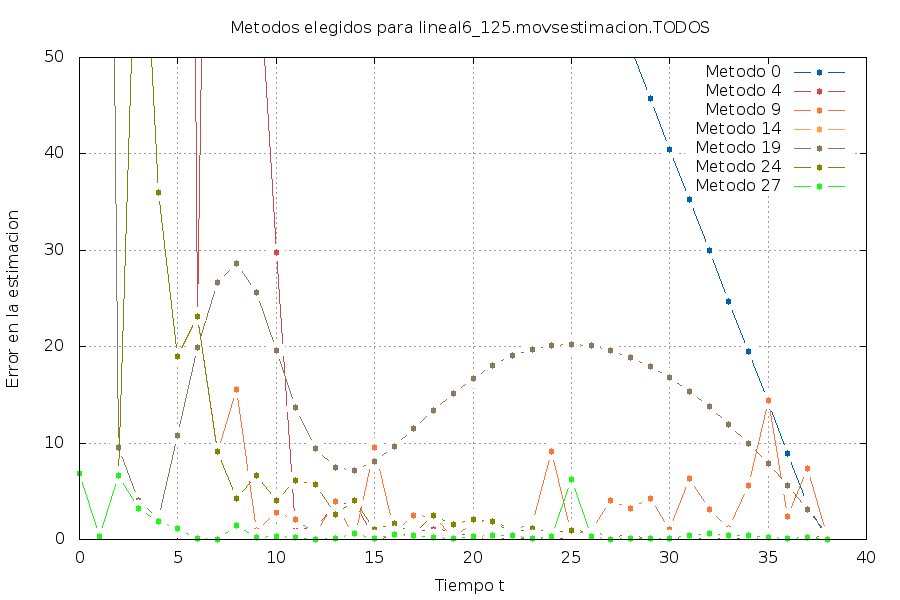
\includegraphics[width=0.9\textwidth]{img/lineal6_125_movsestimacion_TODOS_elegidos.png}
     \caption{ESTIMACION de tiro lineal6}
\end{center}
\end{figure}

\begin{figure}[H]
\begin{center}
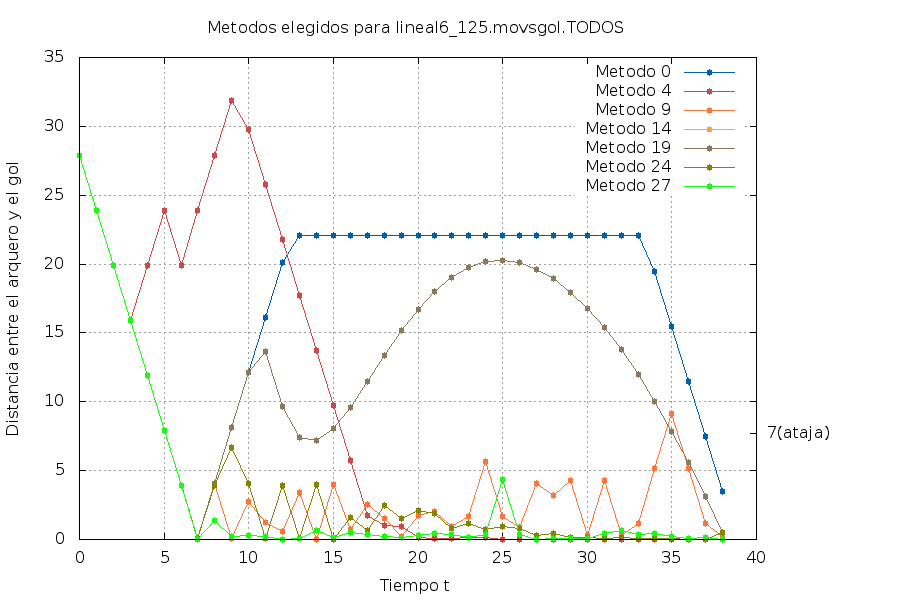
\includegraphics[width=0.9\textwidth]{img/lineal6_125_movsgol_TODOS_elegidos.png}
     \caption{MOVSGOL de tiro lineal6}
\end{center}
\end{figure}


\begin{figure}[H]
\begin{center}
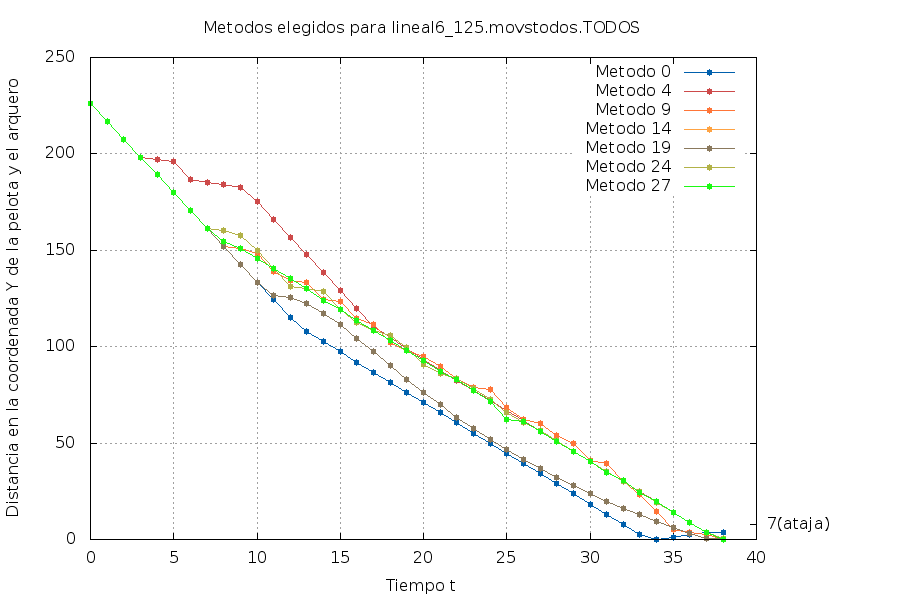
\includegraphics[width=0.9\textwidth]{img/lineal6_125_movstodos_TODOS_elegidos.png}
     \caption{MOVSTODOS de tiro lineal6}
\end{center}
\end{figure}

\textbf{Error estimación:} Se ve que todos mientras mas datos tienen mas chico es el error de
estimacion. Lo que cambia entre los métodos es cuán rápido minimizan el error.
Además se puede ver que todos presentan saltos muy empinados en mayor en o menor medida.
\textbf{Distancia a la posición final de la pelota}:
En el segundo gráfico confirmamos lo visto en el primero dado que miden cosas parecidas pero vistas
desde otra perspectiva. Aunque en todos los métodos nuestro arquero tiende a acercarce a la posición
final de la pelota a medida que pasa el tiempo.
\textbf{Distancia entre el eye Y de la pelota y el arquero:}
Este tercer gráfico también es consistente con los anteriores dado que la distancia en el eje y
entre la pelota y el arquero es siempre decreciente a medida que pasa el tiempo.



\subsection{Experimentacion con Curvas}
%%--------------------------------------------

\subsubsection{Utilizando cuadr3.tiro}

\begin{figure}[H]
\begin{center}
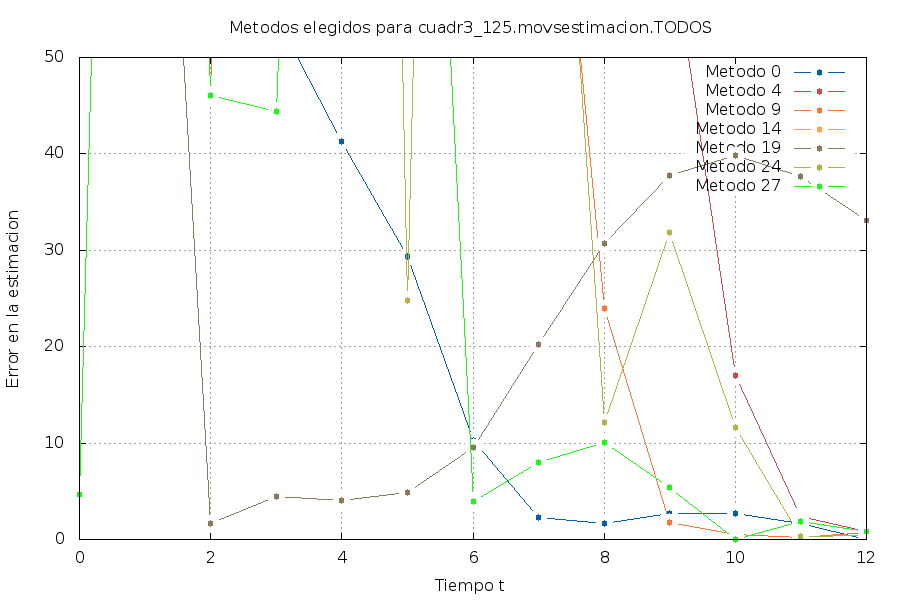
\includegraphics[width=0.9\textwidth]{img/cuadr3_125_movsestimacion_TODOS_elegidos.png}
     \caption{Estimacion de tiro cuadr3}
\end{center}
\end{figure}

\begin{figure}[H]
\begin{center}
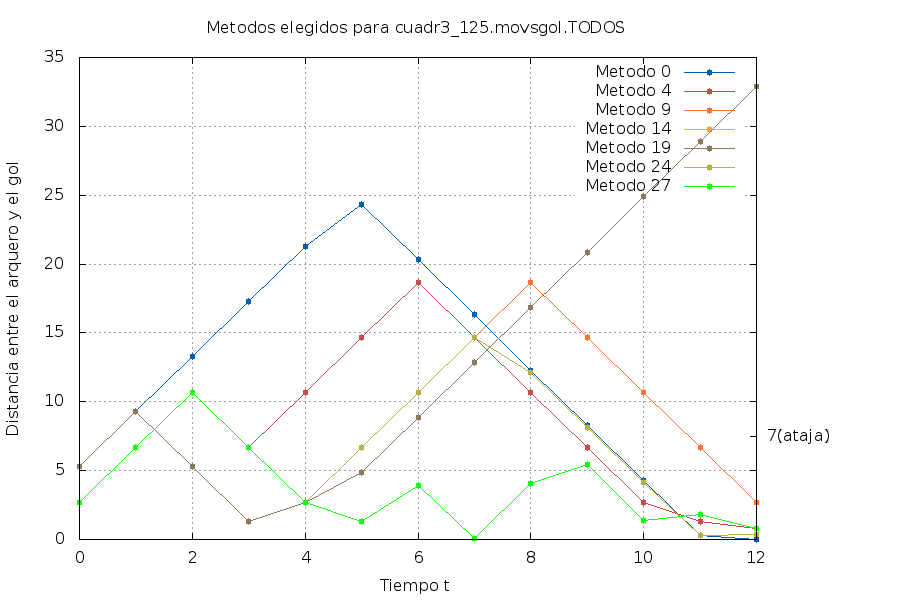
\includegraphics[width=0.9\textwidth]{img/cuadr3_125_movsgol_TODOS_elegidos.png}
     \caption{MOVSGOL de tiro cuadr3}
\end{center}
\end{figure}


\begin{figure}[H]
\begin{center}
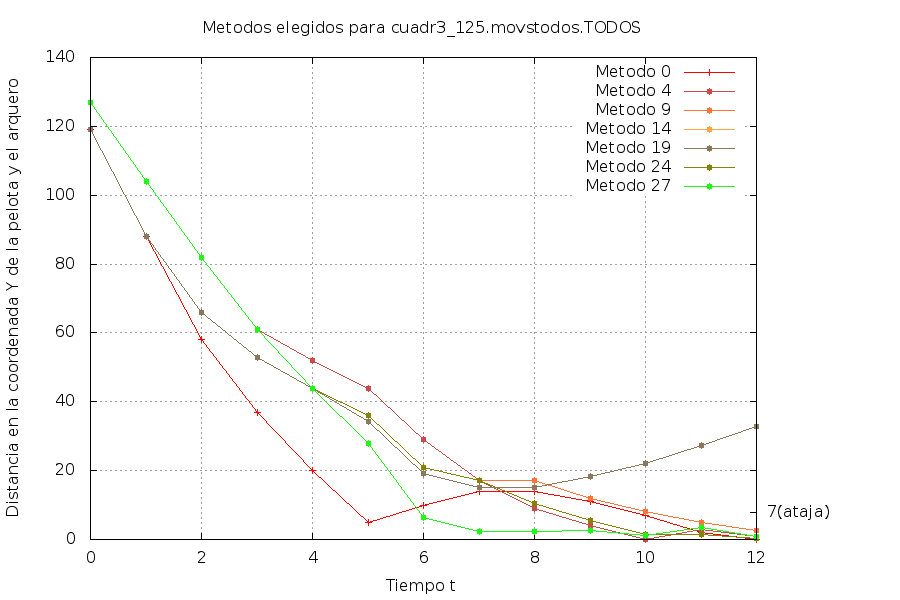
\includegraphics[width=0.9\textwidth]{img/cuadr3_125_movstodos_TODOS_elegidos.png}
     \caption{MOVSTODOS de tiro cuadr3}
\end{center}
\end{figure}

Este tiro corresponde a una curva que describe una función polinómica cuadrática.

Estudiando el error de la estimacion vemos que al ser la curva cuadratica las primeras estimaciones
nos dan datos confusos indicando que la pelota no se esta acercando al arco. A medida que tomamos
datos y superamos el punto critico estas empiezan a tender a la posicion final.

En este tiro aparecio el primer metodo que no logra atajar (metodo 19) indicando que agregar un
supuesto a la estimacion de cuadrados minimos puede traer consecuencias negativas.




%%--------------------------------------------
\subsubsection{Utilizando cuadr6.tiro}

\begin{figure}[H]
\begin{center}
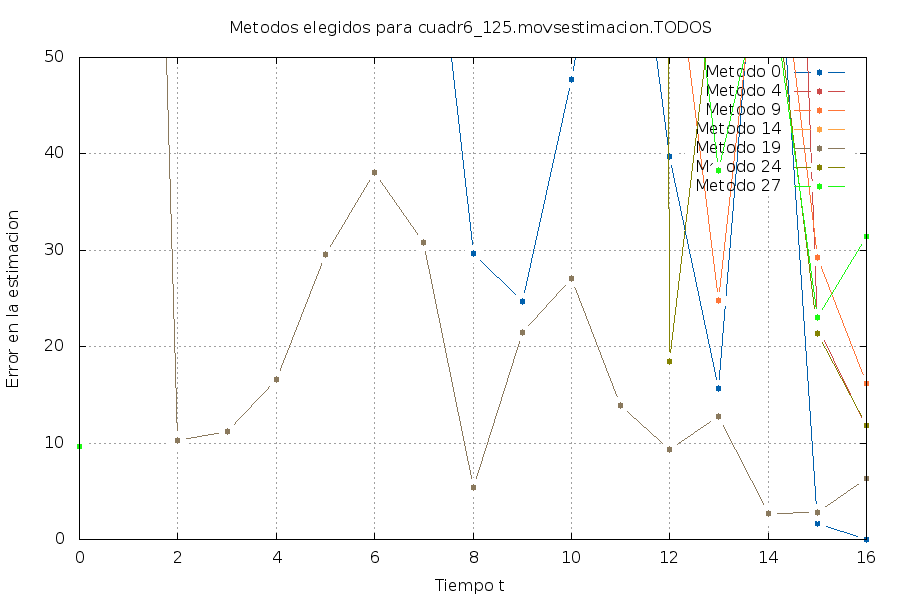
\includegraphics[width=0.9\textwidth]{img/cuadr6_125_movsestimacion_TODOS_elegidos.png}
     \caption{Estimacion de tiro cuadr6}
\end{center}
\end{figure}

\begin{figure}[H]
\begin{center}
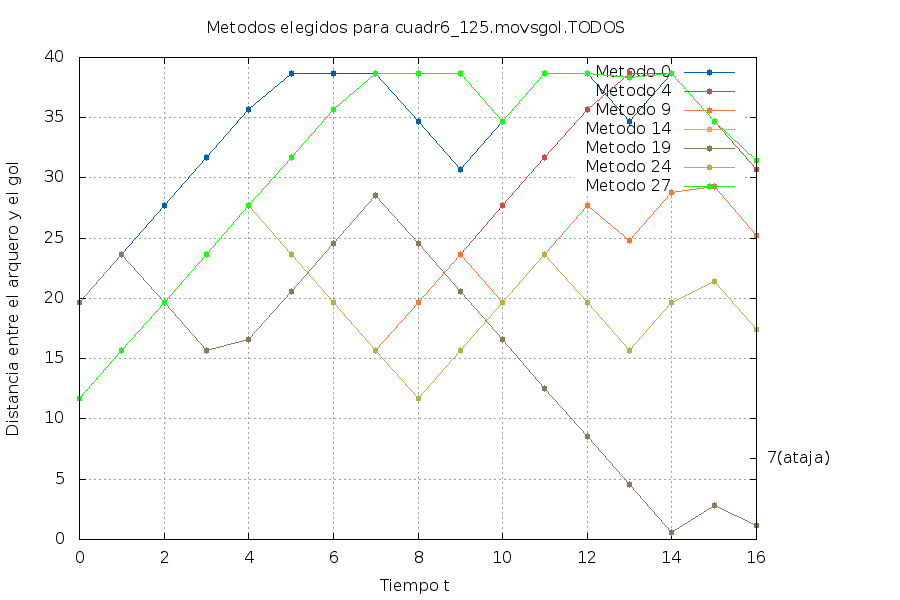
\includegraphics[width=0.9\textwidth]{img/cuadr6_125_movsgol_TODOS_elegidos.png}
     \caption{MOVSGOL de tiro cuadr6}
\end{center}
\end{figure}

\begin{figure}[H]
\begin{center}
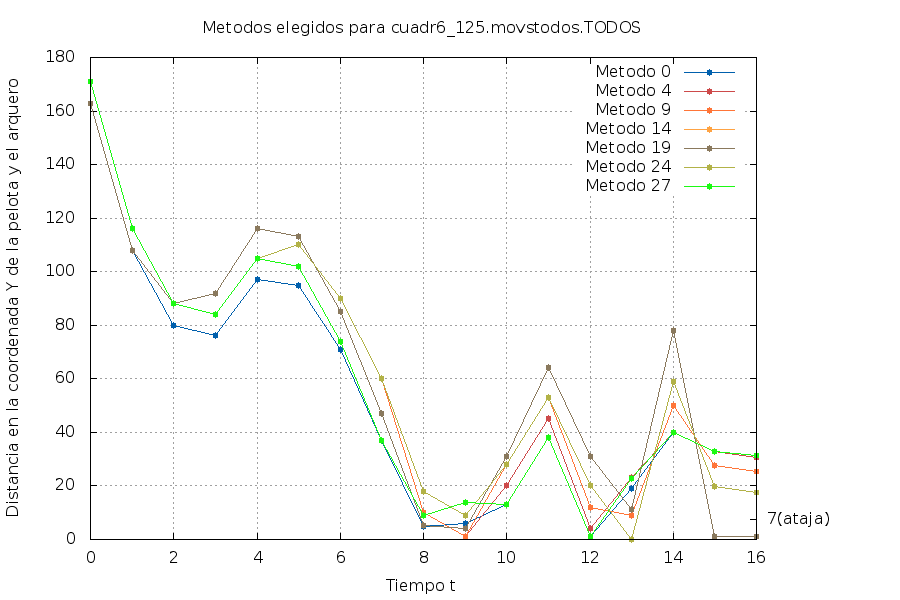
\includegraphics[width=0.9\textwidth]{img/cuadr6_125_movstodos_TODOS_elegidos.png}
     \caption{MOVSTODOS de tiro cuadr6}
\end{center}     
\end{figure}

Este caso es una función muy cambiante por lo que nuestro arquero no logra estimarlo correctamente.
Lo que nos sorprendió fue que hubo un método de los elegidos que si pudo atajarlo, que fue el metodo
19. De los no elegidos, tambien sorprendentemete hubo muchos que pudieron atajarlo si miramos la
tabla. Queda para proximas investigaciones ver el porque.



%%--------------------------------------------
%%--------------------------------------------
%%--------------------------------------------
\subsection{Experimentacion con Jugadores}


%%--------------------------------------------
\subsubsection{Utilizando conj4.tiro}

\begin{figure}[H]
\begin{center}
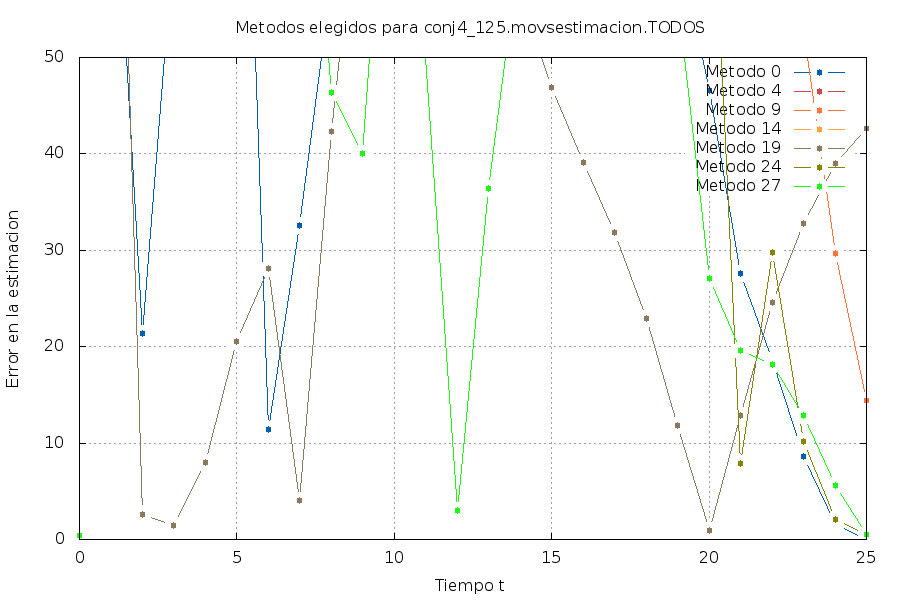
\includegraphics[width=0.9\textwidth]{img/conj4_125_movsestimacion_TODOS_elegidos.png}
     \caption{Estimacion de tiro conj4}
\end{center}
\end{figure}

\begin{figure}[H]
\begin{center}
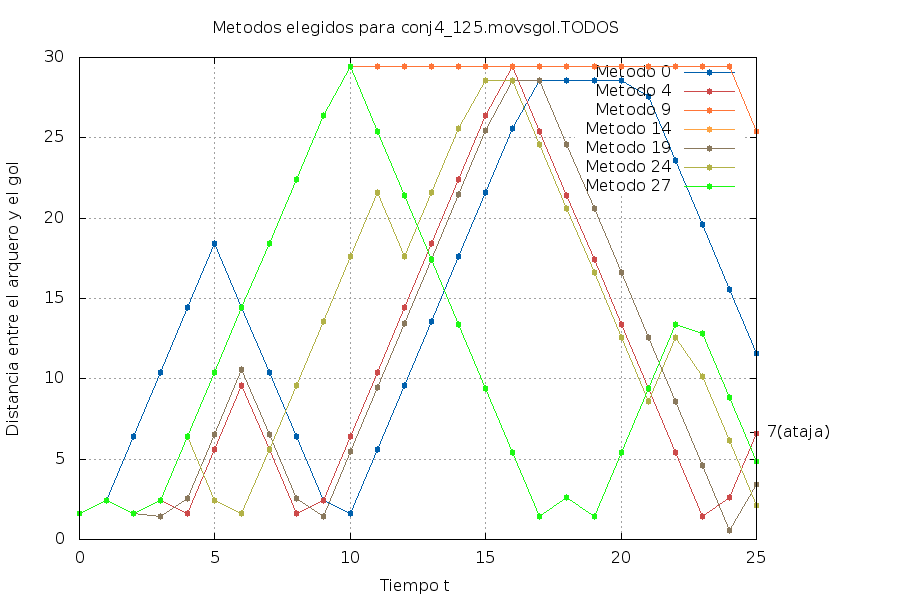
\includegraphics[width=0.9\textwidth]{img/conj4_125_movsgol_TODOS_elegidos.png}
     \caption{MOVSGOL de tiro conj4}
\end{center}
\end{figure}

\begin{figure}[H]
\begin{center}
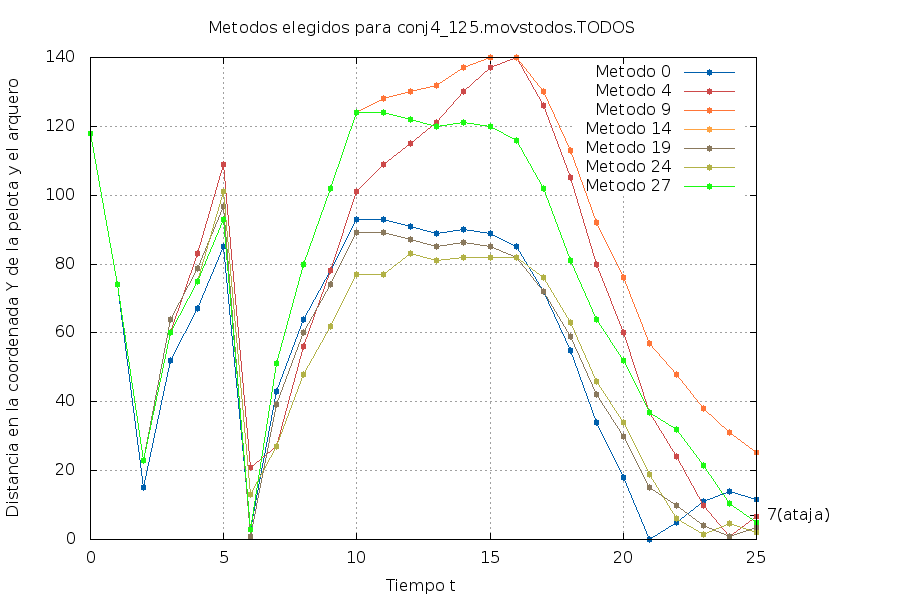
\includegraphics[width=0.9\textwidth]{img/conj4_125_movstodos_TODOS_elegidos.png}
     \caption{MOVSTODOS de tiro conj4}
\end{center}
\end{figure}

En este tiro se producen pasos entre distintos jugadores muy cerca del arco. Lo que observamos es
que cuando se producen pases horizontales se producen picos en los graficos indicando estimaciones
correctas para esa trayectoria temporal.




%%--------------------------------------------
\subsubsection{Utilizando conj8.tiro}

\begin{figure}[H]
\begin{center}
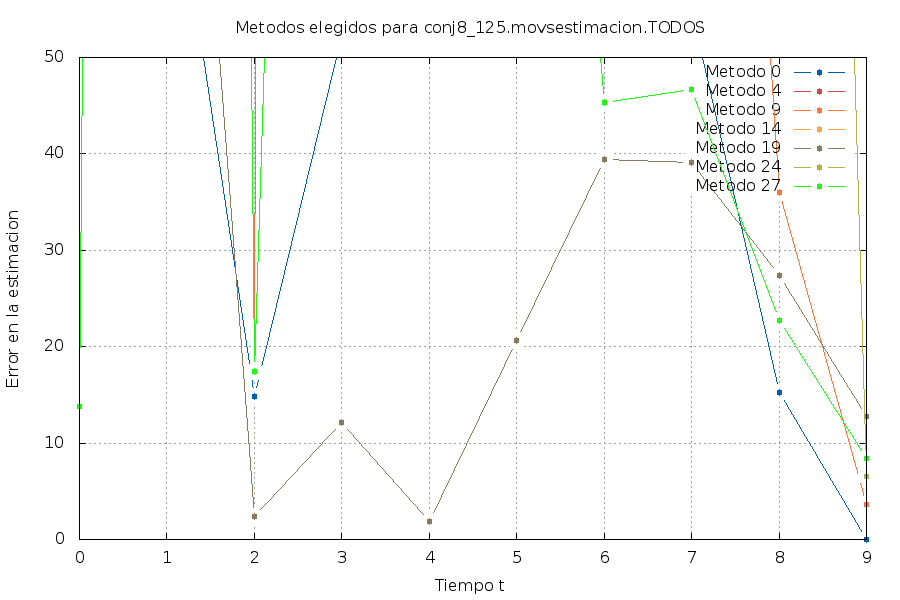
\includegraphics[width=0.9\textwidth]{img/conj8_125_movsestimacion_TODOS_elegidos.png}
     \caption{Estimacion de tiro conj8}
\end{center}
\end{figure}

\begin{figure}[H]
\begin{center}
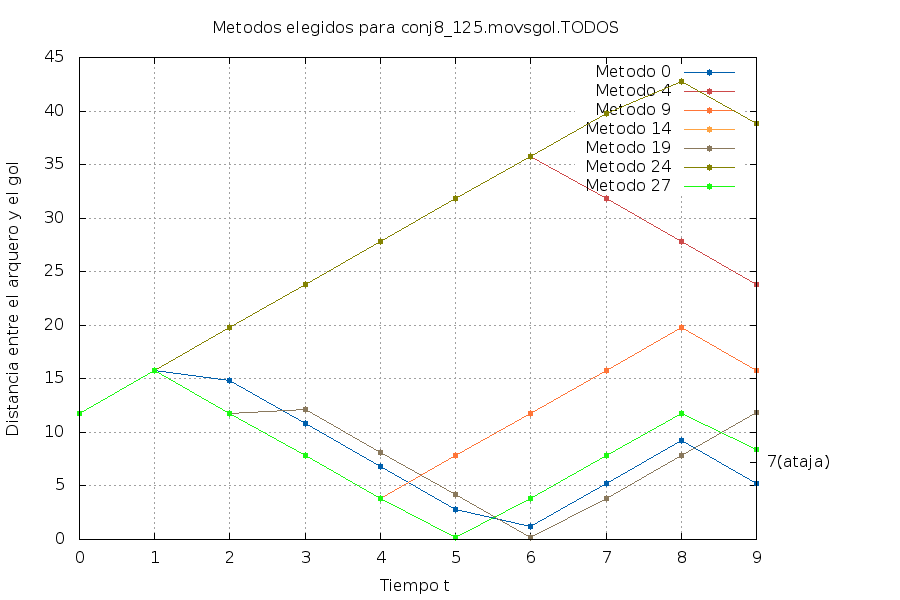
\includegraphics[width=0.9\textwidth]{img/conj8_125_movsgol_TODOS_elegidos.png}
     \caption{MOVSGOL de tiro conj8}
\end{center}
\end{figure}

\begin{figure}[H]
\begin{center}
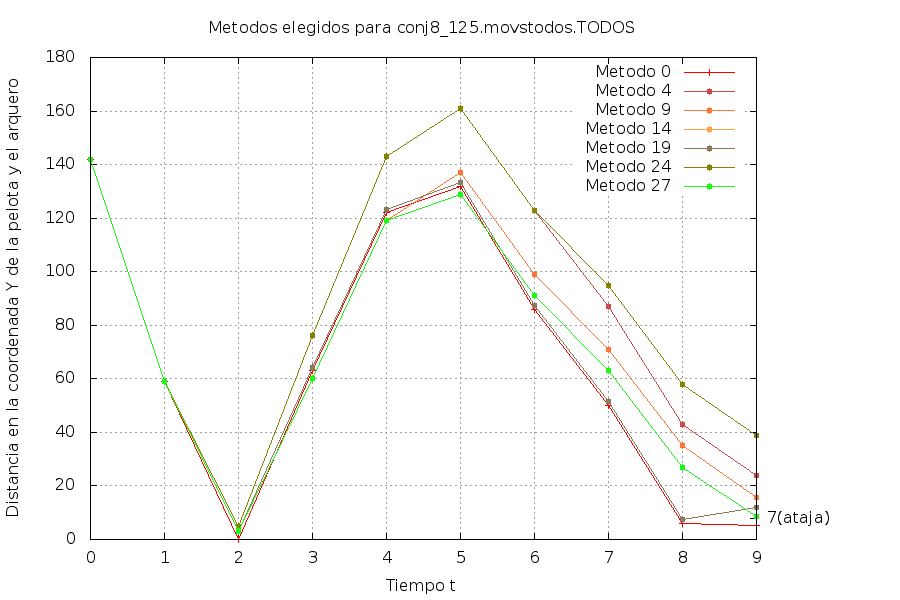
\includegraphics[width=0.9\textwidth]{img/conj8_125_movstodos_TODOS_elegidos.png}
     \caption{MOVSTODOS de tiro conj8}
\end{center}
\end{figure}

En este tiro se produce un pase horizontal pegado al area chica y luego un remate al arco. Es por
eso que notamos un pico muy brusco en los graficos. 


%%--------------------------------------------
%%--------------------------------------------
%%--------------------------------------------
\subsection{Experimentacion con Exoticos}

%%--------------------------------------------
\subsubsection{Utilizando ex5.tiro}

\begin{figure}[H]
\begin{center}
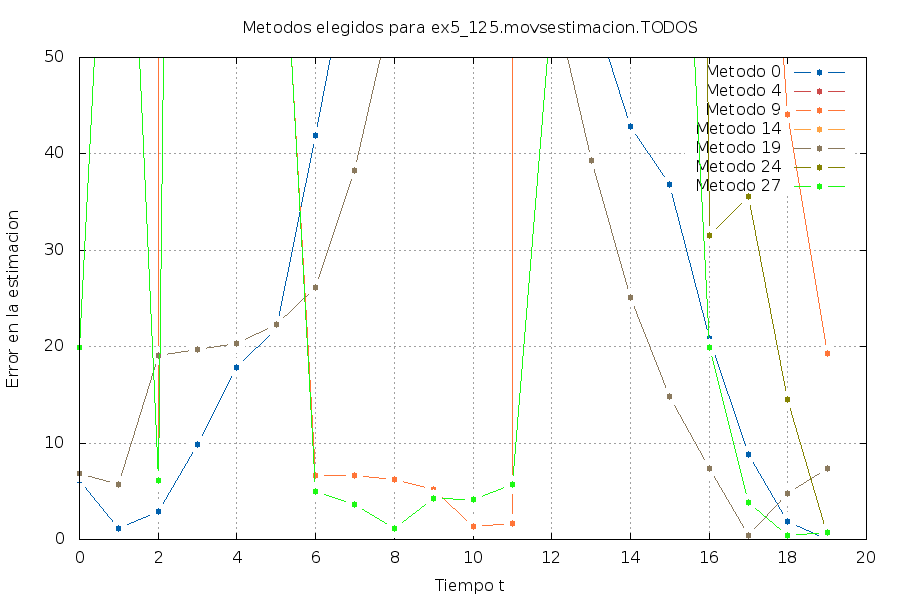
\includegraphics[width=0.9\textwidth]{img/ex5_125_movsestimacion_TODOS_elegidos.png}
     \caption{Estimacion de tiro ex5}
\end{center}
\end{figure}

\begin{figure}[H]
\begin{center}
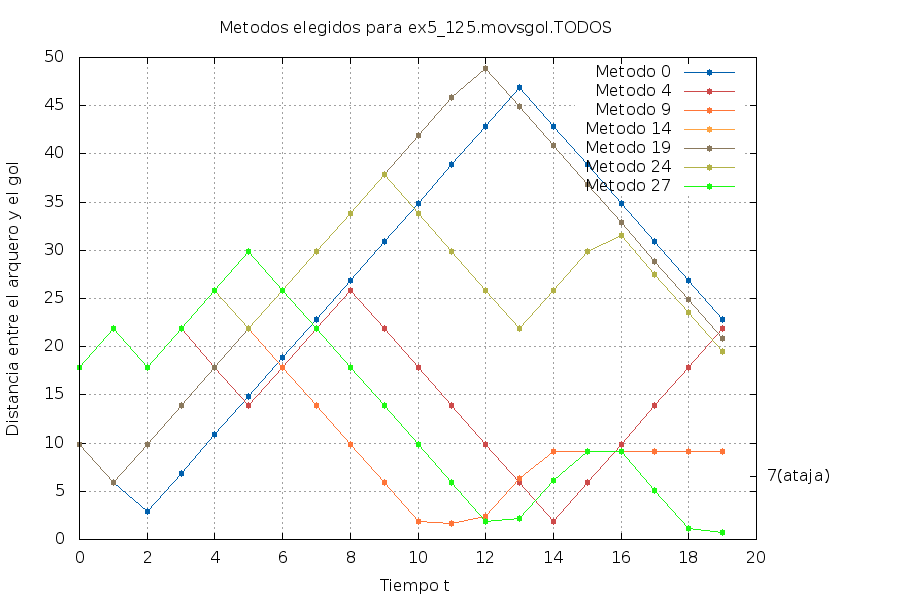
\includegraphics[width=0.9\textwidth]{img/ex5_125_movsgol_TODOS_elegidos.png}
     \caption{MOVSGOL de tiro ex5}
\end{center}
\end{figure}

\begin{figure}[H]
\begin{center}
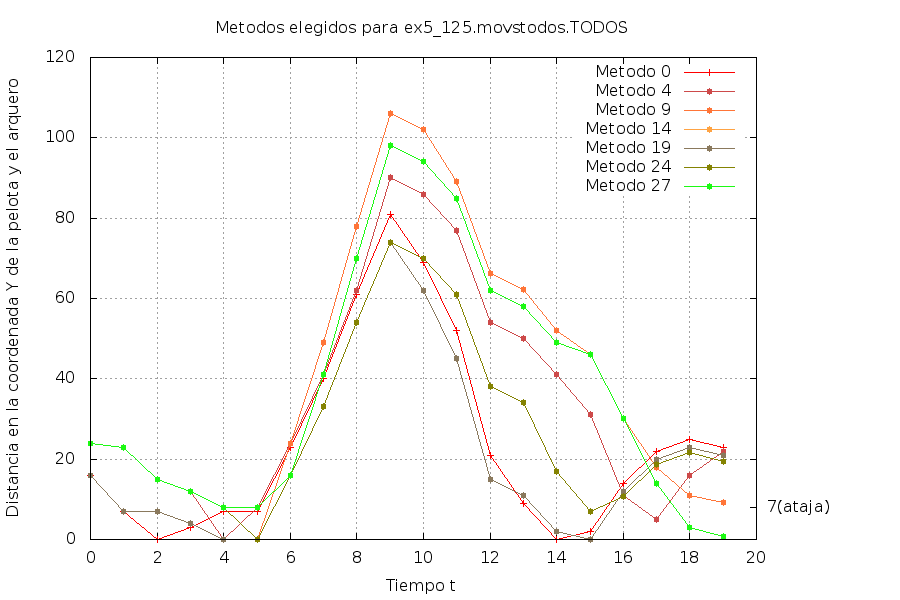
\includegraphics[width=0.9\textwidth]{img/ex5_125_movstodos_TODOS_elegidos.png}
     \caption{MOVSTODOS de tiro ex5}
\end{center}
\end{figure}

Este tiro se produce un tiro libre con rebote en la barrera y remate de otro jugador. Al igual que
en muchos otros tiros al ocurrir el rebote en la barrera notamos picos bruscos en los gráficos
debido a que se limpia el buffer de muestras en esos momentos. Luego del rebote se produce una curva
en la cual vemos como el arquero tiende a acerce a la posicion final de la pelota.
